% Template for Assignment Reports

\documentclass{article}

\usepackage{fancyhdr} % Required for custom headers
\usepackage{lastpage} % Required to determine the last page for the footer
\usepackage{extramarks} % Required for headers and footers
\usepackage{graphicx,color}
\usepackage{anysize}
\usepackage{amsmath}
% \usepackage{natbib}
\usepackage{caption}
\usepackage[hidelinks]{hyperref}
\usepackage{listings,fancyvrb}
\lstset{
  basicstyle=\ttfamily,
  columns=fullflexible,
  frame=single,
  breaklines=true,
  postbreak=\mbox{\textcolor{red}{$\hookrightarrow$}\space},
}
\usepackage{float}
\usepackage{lipsum}  
\usepackage{nameref}
\usepackage{pgf-umlsd}
\usepackage{subcaption}

% Margins
%\topmargin=-0.45in
%\evensidemargin=0in
%\oddsidemargin=0in
\textwidth=6.5in
%\textheight=9.0in
%\headsep=0.25in 
\renewcommand{\familydefault}{\sfdefault}
\usepackage[T1]{fontenc}

\linespread{1.0} % Line spacing

%%------------------------------------------------
%% Image and Listing code
%%------------------------------------------------
%%sw \includecode{caption for table of listings}{caption for reader}{filename}
\newcommand{\includecode}[3]{\lstinputlisting[float,floatplacement=H, caption={[#1]#2}, captionpos=b, frame=single]{#3}}


%%sw \includescalefigure{label}{short caption}{long caption}{scale}{filename}
\newcommand{\includescalefigure}[5]{
\begin{figure}[htb]
\centering
\includegraphics[width=#4\linewidth]{#5}
\captionsetup{width=.8\linewidth} 
\caption[#2]{#3}
\label{#1}
\end{figure}
}

%%sw \includefigure{label}{short caption}{long caption}{filename}
\newcommand{\includefigure}[4]{
\begin{figure}[htb]
\centering
\includegraphics{#4}
\captionsetup{width=.8\linewidth} 
\caption[#2]{#3}
\label{#1}
\end{figure}
}


%%------------------------------------------------
%% Parameters
%%------------------------------------------------
% Set up the header and footer
\pagestyle{fancy}
\lhead{\authorName} % Top left header
\chead{\moduleCode\ - \assignmentTitle} % Top center header
\rhead{\firstxmark} % Top right header
\lfoot{\lastxmark} % Bottom left footer
\cfoot{} % Bottom center footer
\rfoot{Page\ \thepage\ of\ \pageref{LastPage}} % Bottom right footer
\renewcommand\headrulewidth{0.4pt} % Size of the header rule
\renewcommand\footrulewidth{0.4pt} % Size of the footer rule
\setlength\parindent{0pt} % Removes all indentation from paragraphs

\newcommand{\assignmentTitle}{Assignment 1: File Retrieval Protocol} % Assignment title
\newcommand{\moduleCode}{CSU33031} 
\newcommand{\moduleName}{Computer\ Networks} 
\newcommand{\authorName}{Liam\ Junkermann} % Your name
\newcommand{\authorID}{19300141} % Your student ID
\newcommand{\reportDate}{\printDate}
\newcommand{\code}[1]{\texttt{#1}}

%%------------------------------------------------
%%	Title Page
%%------------------------------------------------
\title{
\vspace{-1in}
\begin{figure}[!ht]
\flushleft

\includegraphics[width=0.4\linewidth]{reduced-trinity.png}
\end{figure}
\vspace{-0.5cm}
\hrulefill \\
\vspace{0.5cm}
\textmd{\textbf{\moduleCode\ \moduleName}}\\
\textmd{\textbf{\assignmentTitle}}\\
\vspace{0.5cm}
\hrulefill \\
}

\author{\textbf{\authorName,\ \authorID}}

\date{\today}



%%------------------------------------------------
%% Document
%%------------------------------------------------
\begin{document}
\lstset{language=Java, captionpos=b, frame=single, keywordstyle=\color{black}\bfseries, stringstyle=\ttfamily}
\captionsetup{width=.8\linewidth} 

\maketitle
\tableofcontents
\vspace{0.5in}

\begin{abstract}
	This report will discuss the implementation of a file retrieval protocol. Starting with a brief overview of a protocol which was used as inspiration, the components of the final implementation, an example of a network topology employing this implementation of the protocol, a brief discussion of potential improvements, and finally a summary and reflection of the assignment.
\end{abstract}

\newpage
%%------------------------------------------------
\section{Introduction}

%% The introduction should describe the general problem that should be addressed in the assignment, the approach that you have taken 

For this assignment, a network containing one ingress server connecting a number of clients and workers, working together to request and provide files, was described. Files are to be requested from a \code{Client} via the \code{Ingress} node, the \code{Ingress} node then forwards that request to a worker, the worker then sends the file in response which is also forwarded through the \code{Ingress} node.

In this report I will discuss the inspiration for my solution followed by an explanation of overall design of the network, each element of the solution, and a description of the data packets and content transferred across the network.

%%------------------------------------------------
\section{Theory}


%% The section on the theory at the basis of the assignment should describe the concepts and protocols that were used to realise a solution.

At its core, this file retrieval network is a load balancer for file retrieval workers using multiplexed transport over UDP (User Datagram Protocol). QUIC ({\bf Q}uick {\bf U}DP {\bf I}nternet {\bf C}onnections) Protocol\footnote[1]{\href{https://www.chromium.org/quic/}{https://www.chromium.org/quic/}} is a protocol which implements this concept of multiplexed transport over UDP. A cursory understanding of this protocol provides the basis for a file retrieval protocol which handles multiple sized files as well as basic errors such as packet loss.


%%------------------------------------------------
\subsection{QUIC Protocol}

QUIC was designed to improve page load times, while maintaining secure transport, as an alternative to TCP (Transport Control Protocol) + TLS (Transport Layer Security) + HTTP/2 (Hypertext Transport Protocol/2.0). QUIC was designed to be built on top of UDP as UDP does not suffer from the restrictions imposed by TCP protocols requiring system kernel operation, for example. Due to being built on top of UDP secure connections are maintained and other features are available such as:
\begin{itemize}
	\item Reduced connection establishment time - 0 round trips in the common case
	\item Improved congestion control feedback
	\item Multiplexing without head of line blocking
	\item Connection migration
	\item Transport extensibility
	\item Optional unreliable delivery \cite{QUIC}
\end{itemize}

QUIC operates by establishing a single roundtrip handshake with a client, providing the client with the details to make future requests. From then on QUIC generally needs zero-roundtrips before sending future payloads. QUIC is able to maximise throughput by leveraging UDP's unreliability. Where TCP requires data streams to complete, UDP is nearly expected to lost packets. As a result QUIC is able to handle multiple requests without being blocked by the TCP head-of-line blocking. \cite{QUIC_RFC}

%%------------------------------------------------
\section{Implementation}
\subsection{Overview}
This protocol uses a similar approach to QUIC to handle file responses and requests with a UDP protocol which utilises basic handshake mechanisms to achieve a basic protocol. This has been implemented using three components, configured in a virtual network. These components are an \code{\nameref{subsec:Ingress}}, a \code{\nameref{subsec:Worker}}, and a\code{\nameref{subsec:Client}}. A network would contain one \code{Ingress} node, one to many \code{Worker} nodes, and zero to many \code{Client} nodes. On startup \code{Worker} and \code{Client} nodes register with the \code{Ingress} which then enables the \code{Client}s and \code{Worker}s to interact more efficiently.
\subsubsection[Packet]{Packet Overview}

The base packets have a two byte header where byte 0 is the packet type, and byte one is the source index. Byte one is not always used. The packet types, with their respective value are listed below
\begin{lstlisting}[language=java,caption={[Encoded Packet Types]Code snippet from \code{Node} with the encoded packet types},label={lst:packet_types}]
    // Packet Types
    static final byte FILEREQ = 0;
    static final byte FWDFILEREQ = 1;
    static final byte FILERES = 2;
    static final byte ERRPKT = 3;
    static final byte REGCLIENT = 4;
    static final byte REGWORKER = 5;
    static final byte REGACK = 6;
    static final byte FWDFILERES = 7;
    static final byte FILERESACK = 8;
\end{lstlisting}

All packets transmitted through this network follow a packet structure detailed in \autoref{fig:std_pkt}.
\begin{figure}[!ht]
	\centering
	\begin{BVerbatim}
	 0                   1                   2                   3  
	 0 1 2 3 4 5 6 7 8 9 0 1 2 3 4 5 6 7 8 9 0 1 2 3 4 5 6 7 8 9 0 1
	+---------------------------------------------------------------+
	|                 |               |                             |
	|   PACKET TYPE   |  SOURCE IDX   |                             |
	|                 |               |                             |
	+---------------------------------+                             |
	|                                                               |
	|                            PAYLOAD                            |
	|                                                               |
	+---------------------------------------------------------------+
	\end{BVerbatim}
	\caption{Standard Packet}
	\label{fig:std_pkt}
\end{figure}

There is additional information encoded into the file response packet (\code{FILERES} and \code{FWDFILERES}) payload. 
In order to support files requiring multiple packets to send some extra information must be included with the file byte array content, therefore each payload has a 3 byte "header" of sorts. This "header" includes the sequenceNumber shifted right 8 bits, the sequence number (twice for error checking), as well as the End of File Flag which indicates to the client to stop expecting packets. This results in a packet describe below:
\begin{figure}[!ht]
	\centering
	\begin{BVerbatim}
	 0                   1                   2                   3  
	 0 1 2 3 4 5 6 7 8 9 0 1 2 3 4 5 6 7 8 9 0 1 2 3 4 5 6 7 8 9 0 1
	+---------------------------------------------------------------+
	|                 |               |               |             |
	|   PACKET TYPE   |  SOURCE IDX   |sequenceNo >> 8|  sequenceNo |
	|                 |               |               |             |
	+---------------------------------------------------------------+
	|                 |                                             |
	|    EOF FLAG     |                   PAYLOAD                   |
	|                 |                                             |
	+---------------------------------------------------------------+
	\end{BVerbatim}
	\caption{File Response Packet}
\end{figure}
\subsubsection[Operation]{Operation overview}
\autoref{fig:registrations} and \autoref{fig:file_transmission} show the processes to register and introduce new nodes to the network, and request and transmit requested files across the network respectively.
\begin{figure}[!ht]
	\centering
	\begin{minipage}{.5\textwidth}
		\centering
		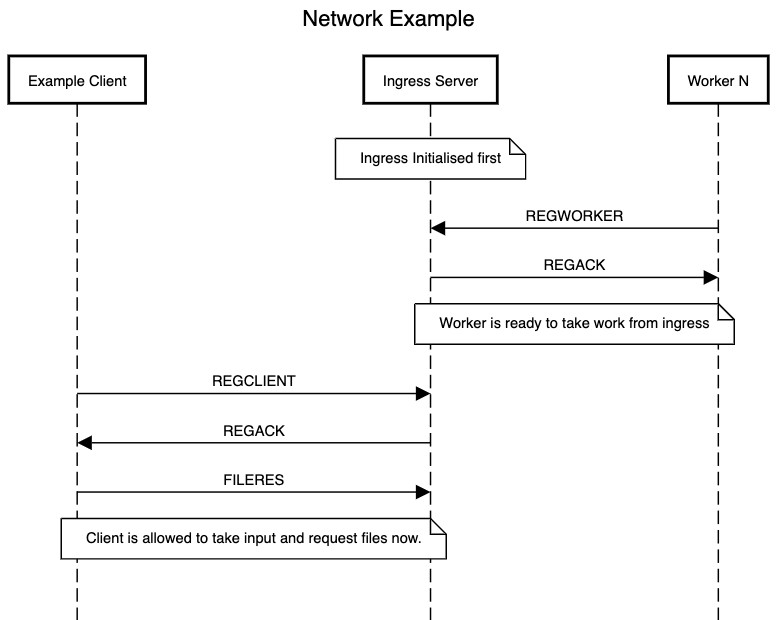
\includegraphics[width=0.8\linewidth]{client-worker-reg.png}
		\captionsetup{width=.6\linewidth}
		\captionof{figure}[\code{Ingress} registration]{Registration of \code{Client} and \code{Worker} nodes to the \code{Ingress} node.}
		\label{fig:registrations}
	\end{minipage}%
	\begin{minipage}{.5\textwidth}
		\centering
		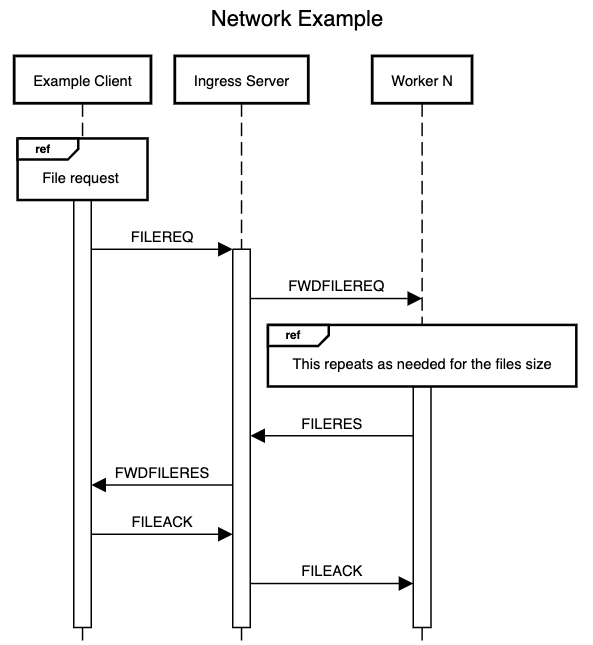
\includegraphics[width=0.8\linewidth]{file_req.png}
		\captionsetup{width=.6\linewidth}
		\captionof{figure}[File transmission]{The sequence diagram detailing the process of requesting and transmitting files.}
		\label{fig:file_transmission}
	\end{minipage}
\end{figure}

The implementation of this network allows for efficient communication between workers and clients through the \code{Ingress} node. The use of a map in the \code{Ingress} allows for a more efficient packet header as only 1 byte is needed to keep track of workers and clients. As all the traffic goes through the \code{Ingress} node, it can act as a router without massive impact on performance. The single byte packet header does impose a limit of only being able to serve up to 15 active clients or workers. If a larger network was needed this could be converted to a two byte header for source index to allow up to 255 \code{Client} nodes and \code{Worker} nodes. Given the size of this implementation 15 workers were more than necessary.

\begin{figure}[!ht]
	\centering
	\begin{minipage}{.5\textwidth}
		\centering
		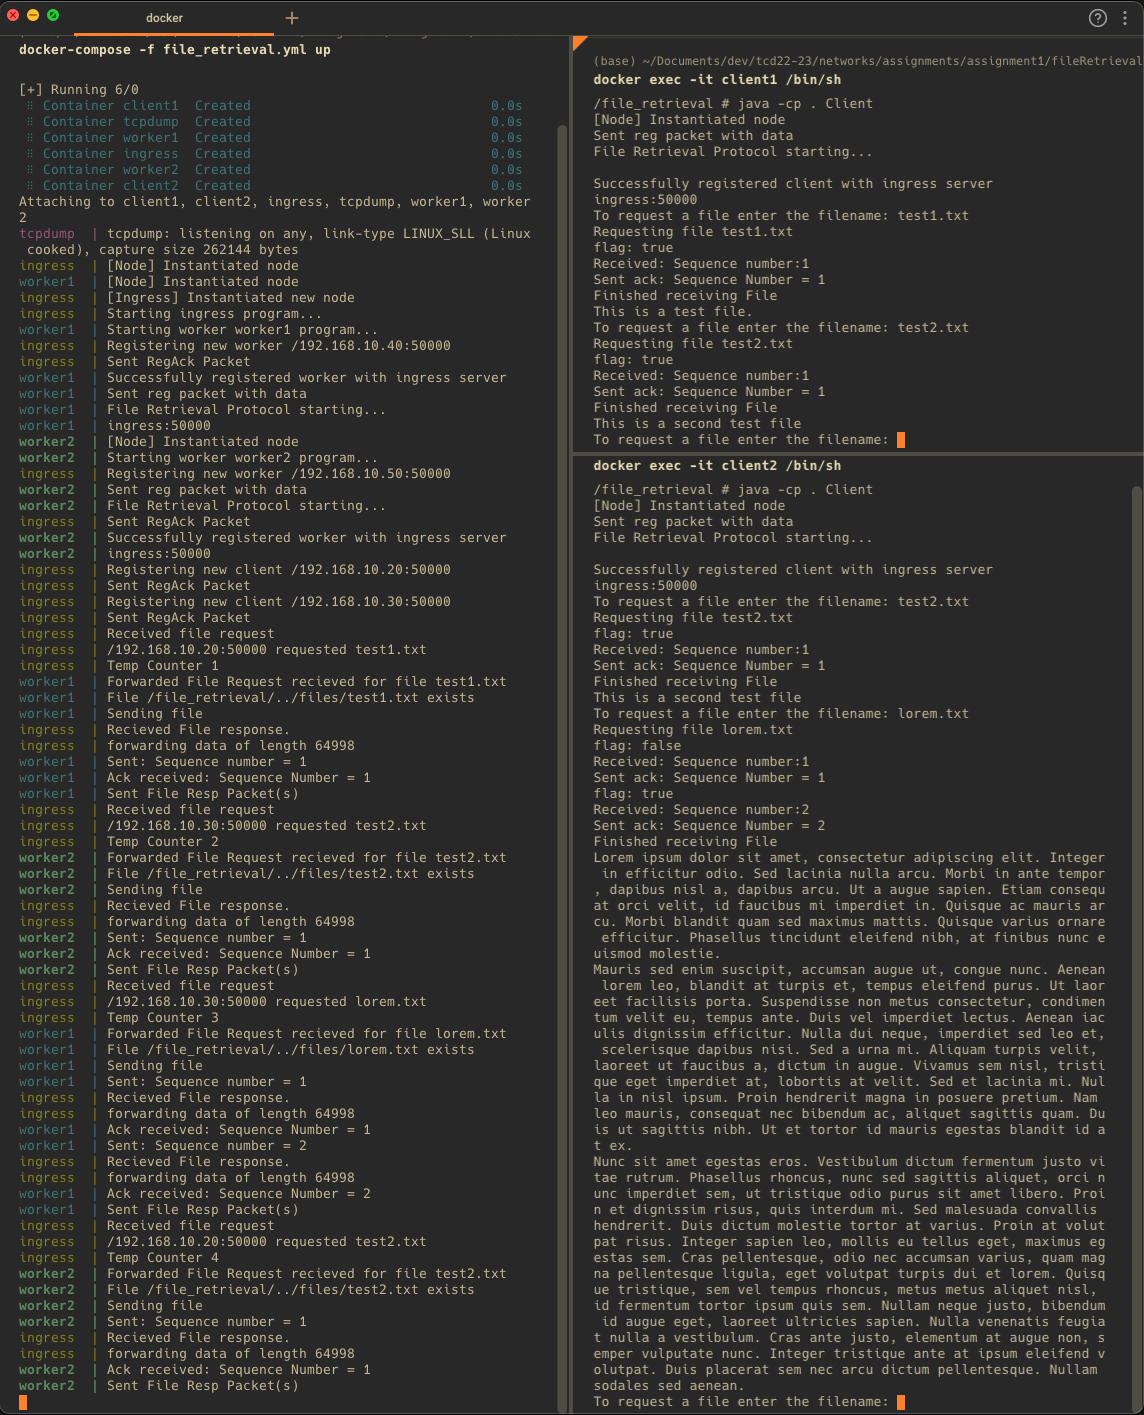
\includegraphics[width=0.8\linewidth]{operation_example.png}
		\captionsetup{width=.75\linewidth}
		\captionof{figure}[Completed network operation]{Client Interactions and logs from headless nodes}
		\label{fig:operation_example}
	\end{minipage}%
	\begin{minipage}{.5\textwidth}
		\centering
		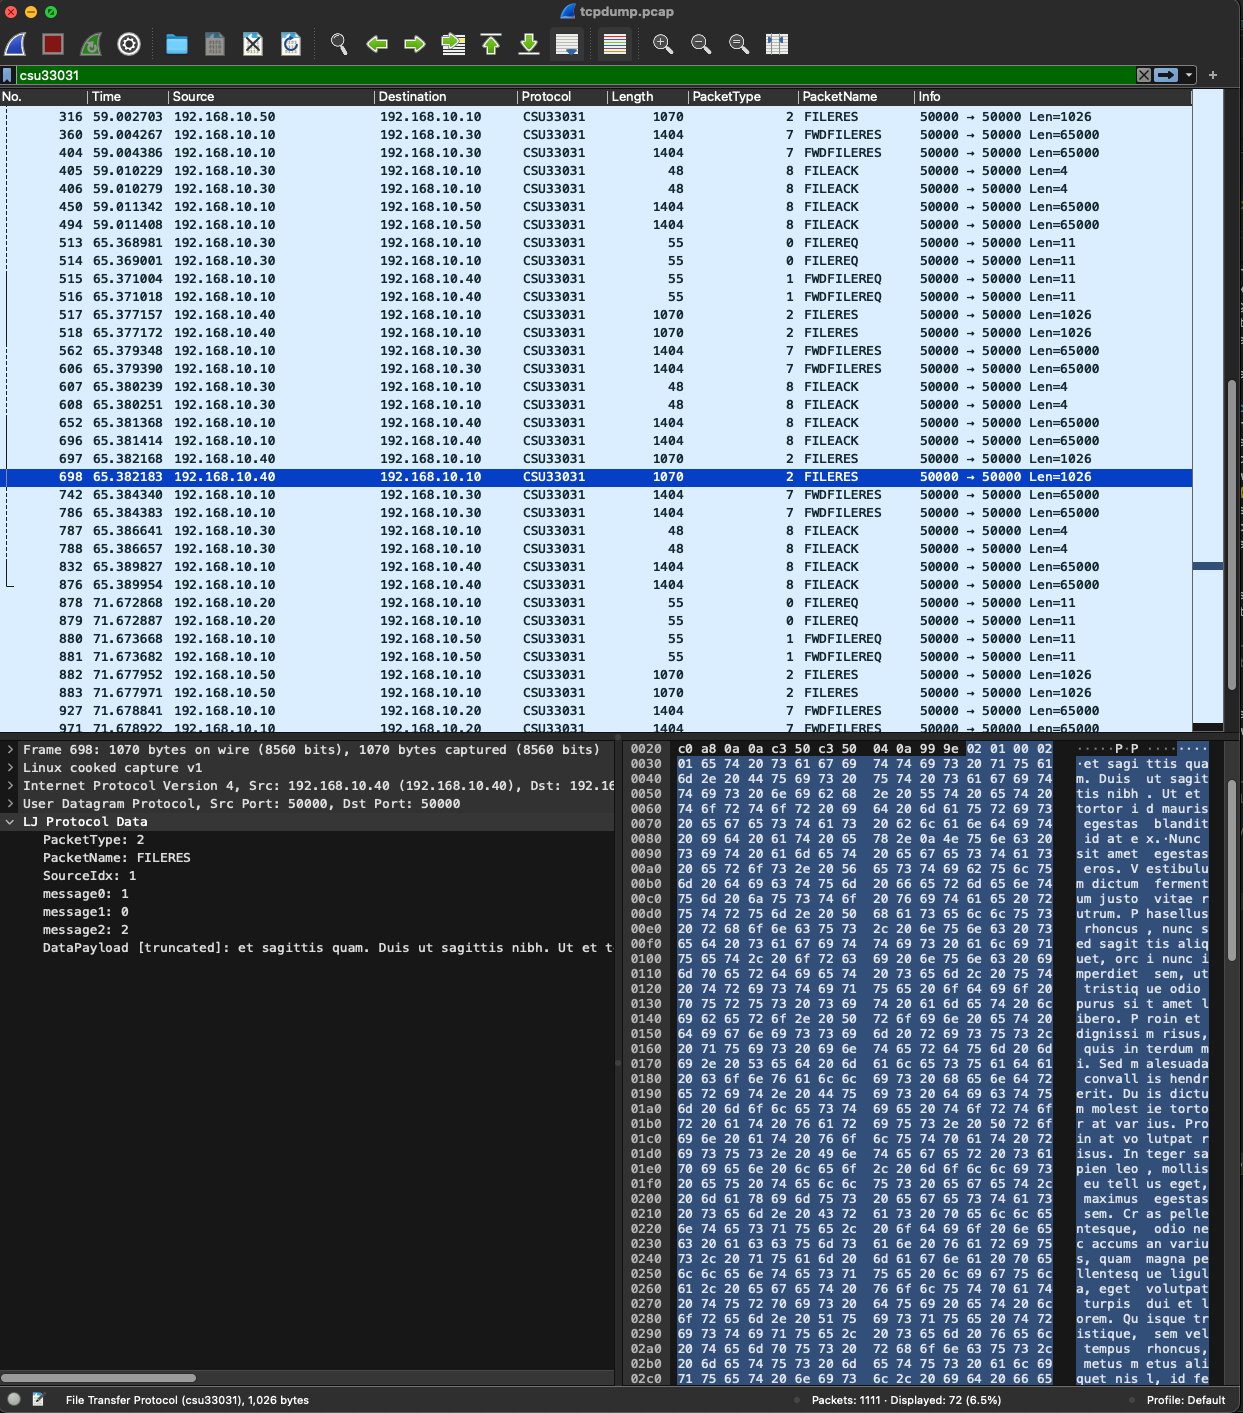
\includegraphics[width=0.8\linewidth]{working_capture.png}
		\captionsetup{width=.75\linewidth}
		\captionof{figure}[PCAP of completed network operation]{The network capture of file transfers between the \code{Worker}, \code{Ingress}, and \code{Client} nodes}
		\label{fig:operation_example_capture}
	\end{minipage}
\end{figure}

\autoref{fig:operation_example} shows an example of the basic operation of the entire network. The left pane shows the logs of the headless nodes (the \code{Ingress} node, and two \code{Worker} nodes). The two panels on the right show the input and output of example \code{Client} nodes.
\autoref{fig:operation_example_capture} shows the block of packets which are doing the actual file transfer. You can see the forwarding of File responses and acknowledgments, as well as a peek into the final packet of the example \code{lorem.txt} file.

\subsection{Network Components}
\subsubsection{Node}
\label{subsec:Node}
In practice each of these network nodes implement a \code{Node} class which handles most of the boilerplate Datagram behaviour and sets constants for header length, values, and positions, as well as providing some worker functions to generate packets and packet data appropriately. This \code{Node} also handles the multithreading needed to successfully multiplex within the \code{\nameref{subsec:Ingress}}.

\subsubsection{Ingress}
\label{subsec:Ingress}
The \code{Ingress} works as a router or proxy. All requests from \code{Client} nodes pass through the \code{Ingress} node and are routed to the relevant \code{Worker} nodes, then again from \code{Worker} to \code{Client}. The \code{Ingress} node must always be the first node to activate as all the other nodes must be registered with the \code{Ingress} node. Registration is done in order to make the packet header a bit slimmer, as previously discussed.
There are generally five packet types supported by the \code{Ingress}:
\begin{description}
	\item[Node Registration] There are two kinds of registration packets: \code{Worker} and \code{Client} registration packets, constants \code{REGWORKER} and \code{REGCLIENT} respectively. The registration packets register the \code{Worker} or \code{Client} in an \code{ArrayList}, the index of which will be used to reference the relevant node in future network events. The use of an \code{ArrayList} allows nodes which may have disconnected, or restarted, to be re-registered without growing an array.
	\item[File Request] The \code{FILEREQ} is a request made from any \code{Client} node which is then processed and forwarded to a \code{Worker} in a \code{FWDFILEREQ} packet which contains information such as the source index to allow the response data to be directed appropriately. The worker is selected using a simple round-robin approach.
	\item[File Response] The \code{FILERES} is the response to a File Request from any \code{Worker} node forwarded to the relevant \code{Client}, based on the \code{ArrayList} index in the header, in a \code{FWDFILERES} packet which includes the workers source index in the header.
	\item[File Response Acknowledgment] The \code{FILERESACK} packet is a key part of the file requesting/response flow. For large files requiring multiple packets to transfer this acknowledgment packet allows the worker handling a given file transfer to progress to transmitting the next packet. The \code{Ingress} node handles this packet by replacing the source index value with the index of the sending \code{Client}, before forwarding the rest of the packet, untouched, to the relevant \code{Worker}.
	\item[Worker Error] Finally, the \code{ERRPKT} is a packet sent from a \code{Worker} node to be forwarded to the \code{Client} node. As will be discussed in the \code{\nameref{subsec:Client}} section, the \code{Client} essentially blocks any input until a request has been completed. If an error occurs in the \code{Worker} this packet is sent, via the \code{Ingress}, to the blocked \code{Client}.
\end{description}
The \code{Ingress} node is a headless node, meaning it does not take user input. As such, it is one of the nodes, when deployed using \href{https://docs.docker.com/compose/}{Docker Compose}\footnote{Docker Compose: https://docs.docker.com/compose/}, which is automatically started when the cluster starts. 
\includescalefigure{fig:ingress_start_log}{Start log of \code{Ingress} Node}{A snippet of the Docker Compose Logs showing the \code{Ingress} node service starting automatically}{1}{ingress_start_log.png}

\subsubsection{Worker}
\label{subsec:Worker}
The \code{Worker} node handles retrieving files from the filesystem based on requests from \code{Client}s via the \code{Ingress}. The main work done by the \code{Worker} node is through the \code{sendFile} function. This function fetches the requested file from the filesystem, converting it to a byte array, then iterating through that byte array in 1021 byte blocks until the end of file, transmitting each block with some extra wrapping to let the \code{Client} know which "sequence" number has been sent, and if the \code{Worker} has reached the end of the byte array. The final \code{FILERES} payload size becomes 1024 bytes with this extra information added. This packet is then wrapped to include the information the ingress needs to forward the data appropriately. The \code{Worker} then waits for the acknowledgment packet to be returned before continuing onto the next packet of data (if applicable).

% \begin{lstlisting}[caption={[File Transmission Code]The code used to generate and send packets based on the file byte array. For the full function please reference the source code}, label={lst:worker_message_gen}, language=java]
% 	for (int i = 0; i < fileByteArray.length; i = i + 1021) {
% 		sequenceNumber += 1;
	
% 		// Create message (this is wrapped by our packets)
% 		byte[] message = new byte[1024]; // First two bytes of the data are for control (datagram integrity and // order)
% 		message[0] = (byte) (sequenceNumber >> 8);
% 		message[1] = (byte) (sequenceNumber);
	
% 		if ((i + 1021) >= fileByteArray.length) { // Have we reached the end of file?
% 			flag = true;
% 			message[2] = (byte) (1); // We reached the end of the file (last datagram to be send)
% 		} else {
% 			flag = false;
% 			message[2] = (byte) (0); // We haven't reached the end of the file, still sending datagrams
% 		}
	
% 		if (!flag) {
% 			System.arraycopy(fileByteArray, i, message, 3, 1021);
% 		} else { // If it is the last datagram
% 			System.arraycopy(fileByteArray, i, message, 3, fileByteArray.length - i);
% 		}
% 		// Remaining code to generate protocol packets and handle acknowledgment before continuing
% 	}
% \end{lstlisting}

The packets which the \code{Worker} node's \code{onReceipt} function handles are:
\begin{description}
	\item[Forwarded File Request] The \code{FWDFILEREQUEST} comes from the \code{\nameref{subsec:Ingress}}, as noted above, and triggers the \code{sendFile} resulting in the behaviour described above.
	\item[Registration Acknowledgment] The \code{REGACK} also comes from the \code{\nameref{subsec:Ingress}} and lets the worker know it is registered.
\end{description}
Just as the \code{Ingress} node is a headless node, so is the \code{Worker} node. As a result both workers get launched automatically when the cluster starts.
\includescalefigure{fig:worker_start_log}{Start log of \code{Worker} nodes}{A snippet of the Docker Compose Logs showing the \code{Worker} node services starting automatically}{1}{worker_start_log.png}

\subsubsection{Client}
\label{subsec:Client}
The \code{Client} node handles taking user input and printing out the result of file requests. Much like the \code{\nameref{subsec:Worker}} the heavy lifting of the function is done by the \code{handleFileRes} function. First, a user enters a filename input. This action triggers a file request to be sent to the \code{Ingress} node and blocks further user input. The \code{handleFileRes} function handles the response packets sent from the \code{Worker} nodes through the \code{Ingress} node, writing the byte content to a buffer until the finished flag has been sent. Once the end of file packet has been sent, the \code{handleFileRes} function then prints out the \code{fileByteArray} in string format, clears the buffer, and unblocks the user input to allow a new file to be requested. While handling the file response packets, the \code{handleFileRes} function validates the packets have been received in the right order, and responds with the appropriate acknowledgment packet.

% \begin{lstlisting}[language=java,caption={[File Receiving Code]The code used to accept file transmissions and print when complete}, label={lst:client_message_receive}] 
% 	byte[] message = getPayloadData(packet);
%         byte[] fileByteArray = new byte[1021];

%         // Retrieve sequence number
%         sequenceNumber = ((message[0] & 0xff) << 8) + (message[1] & 0xff);
%         // Check if we reached last datagram (end of file)
%         flag = (message[2] & 0xff) == 1;
%         System.out.println("flag: " + flag);

%         // If sequence number is the last seen + 1, then it is correct
%         // We get the data from the message and write the ack that it has been received correctly
%         if (sequenceNumber == (foundLast + 1)) {

%             // set the last sequence number to be the one we just received
%             foundLast = sequenceNumber;

%             // Retrieve data from message
%             System.arraycopy(message, 3, fileByteArray, 0, 1021);

%             // Write the retrieved data to the output stream buffer and print received data sequence number
%             outputStream.write(fileByteArray);

%             System.out.println("Received: Sequence number:" + foundLast);

%             // Send acknowledgement
%             sendFileAck(foundLast, socket, packet.getData()[SRC_POS]);
%         } else {
%             System.out.println("Expected sequence number: " + (foundLast + 1) + " but received " + sequenceNumber
%                     + ". DISCARDING");
%             // Re send the acknowledgement
%             sendFileAck(foundLast, socket, packet.getData()[SRC_POS]);
%         }
%         // Check for last datagram
%         if (flag) {
%             System.out.println("Finished receiving File");
%             System.out.println(outputStream.toString());
%             outputStream.flush();
%             blocked = false;
%             return;
%         }
% \end{lstlisting}

The remaining packets handled by the \code{Client} node are:
\begin{description}
	\item[Error Packet] The \code{ERRPKT} packet is sent from the \code{Ingress} node when an error has occurred within the \code{Ingress} or \code{Worker} node for a given transaction. This packet is sent to unblock the \code{Client} so they user may continue by either trying to repeat their request or suggesting them to restart the network.
	\item[Registration Acknowledgment] The \code{REGACK} packet is sent from the \code{Ingress} node to confirm that the \code{Client} has been registered and can request and accept files. 
\end{description}
The \code{Client} node requires user interaction. The current Docker Compose environment creates the virtual machine and a user must start and interact with the Client once the cluster has started.
\includescalefigure{fig:client_example}{Client Example}{An example of a user using the \code{Client}, showing an error, a small single-packet file, and a larger multi-packet file transaction}{0.8}{client1.png}

\section{Future Enhancements}
\label{sec:future_enhancements}
\subsection{Load Balancing}
The \code{Ingress} node also acts as a load balancer for the workers. The load-balancing approach used has much room for improvement. Currently a simple round robin approach is used, iterating a counter with each new file request to select which \code{Worker} to use. This could be improved by being more dynamic with load balancing, including using the forwarded packet sizes, or even the content (has the \code{Worker} sent a packet with an EOF flag in the last \code{x} packets), to determine if a worker is getting requests for larger files. This load balancing approach also does not account for Nodes disconnecting after registration. Having a mechanism to track if a node is still online could be helpful in maintaining \code{Client}/\code{Worker} maps.

\subsection{Node Registration}
The \code{Client} and \code{Worker} nodes could be improved by building a more robust registration process. With the current implementation it is imperative that the \code{Ingress} node is enabled and active before new nodes may be introduced to the network. For the purposes of this project I introduced a \code{sleep} function call to the initialisation of the \code{Worker} nodes, as those are brought online by the docker compose script automatically. The \code{Client} nodes do not need this workaround as they are started manually once the headless nodes activate. 

%%------------------------------------------------
%% Summary of the document i.e. what was presented, what was the outcome of the project and the document.
\section{Summary}
In this report discussed the requirements for the assignment, the real-world version of a solution from which I drew inspiration, and finally my implementation of a file retrieval protocol. Then, an exploration of the basic functionality and an example topology of the completed network, as well as some limitations and potential improvements to this implementation.

%%------------------------------------------------
%% The reflection should layout your thoughts on the assignment
%% How many hours did you spent on the assignment? What worked well for you/what didn't?
%% What would you improve/change in your approach for the next assignment?
\section{Reflection}
This project is relatively large in scope, and having biweekly "check-ins" as blackboard assignments has helped break down the project and remind me to continue working on it at a more manageable pace. While these check-ins were helpful, it was not entirely clear what the objective of each one was and will be something I will clarify for the next project. In general I find it much easier to understand concepts discussed in lectures when I have the opportunity to work with them. Working on this project has given me a better understanding of the basic networks concepts discussed in class, and showed me how a design decision earlier on in the process can have knock-on effects when implementing more advanced features such as file requiring multiple packets to transmit completely. Without including the time needed to write this report this project took me roughly 24 hours to complete. I spent a bit more time earlier on exploring the QUIC protocol to get a better understanding of how to implement a similar solution. In retrospect it may have been more efficient to try and put something together to get a better understanding of the potential problems and iterate on that approach. I noticed I was able to understand the documentation associated with the QUIC protocol much more after completing a version of my solution, based on the learnings I had while building the solution.

\begin{thebibliography}{1}
	\bibitem{QUIC} Google, and Internet Engineering Task Force. “QUIC, a Multiplexed Transport over UDP.” www.chromium.org, Google, 2022, www.chromium.org/quic/.
	\bibitem{QUIC_RFC} Jana Iyengar and Martin Thomson. QUIC: A UDP-Based Multiplexed and Secure Transport. RFC Editor, 2021, doi:10.17487/RFC9000.
\end{thebibliography}

\end{document}